\section{Feature Preserving Curved Shell}\label{cumin:sec:features-pres}


\begin{figure}
    \centering
    % 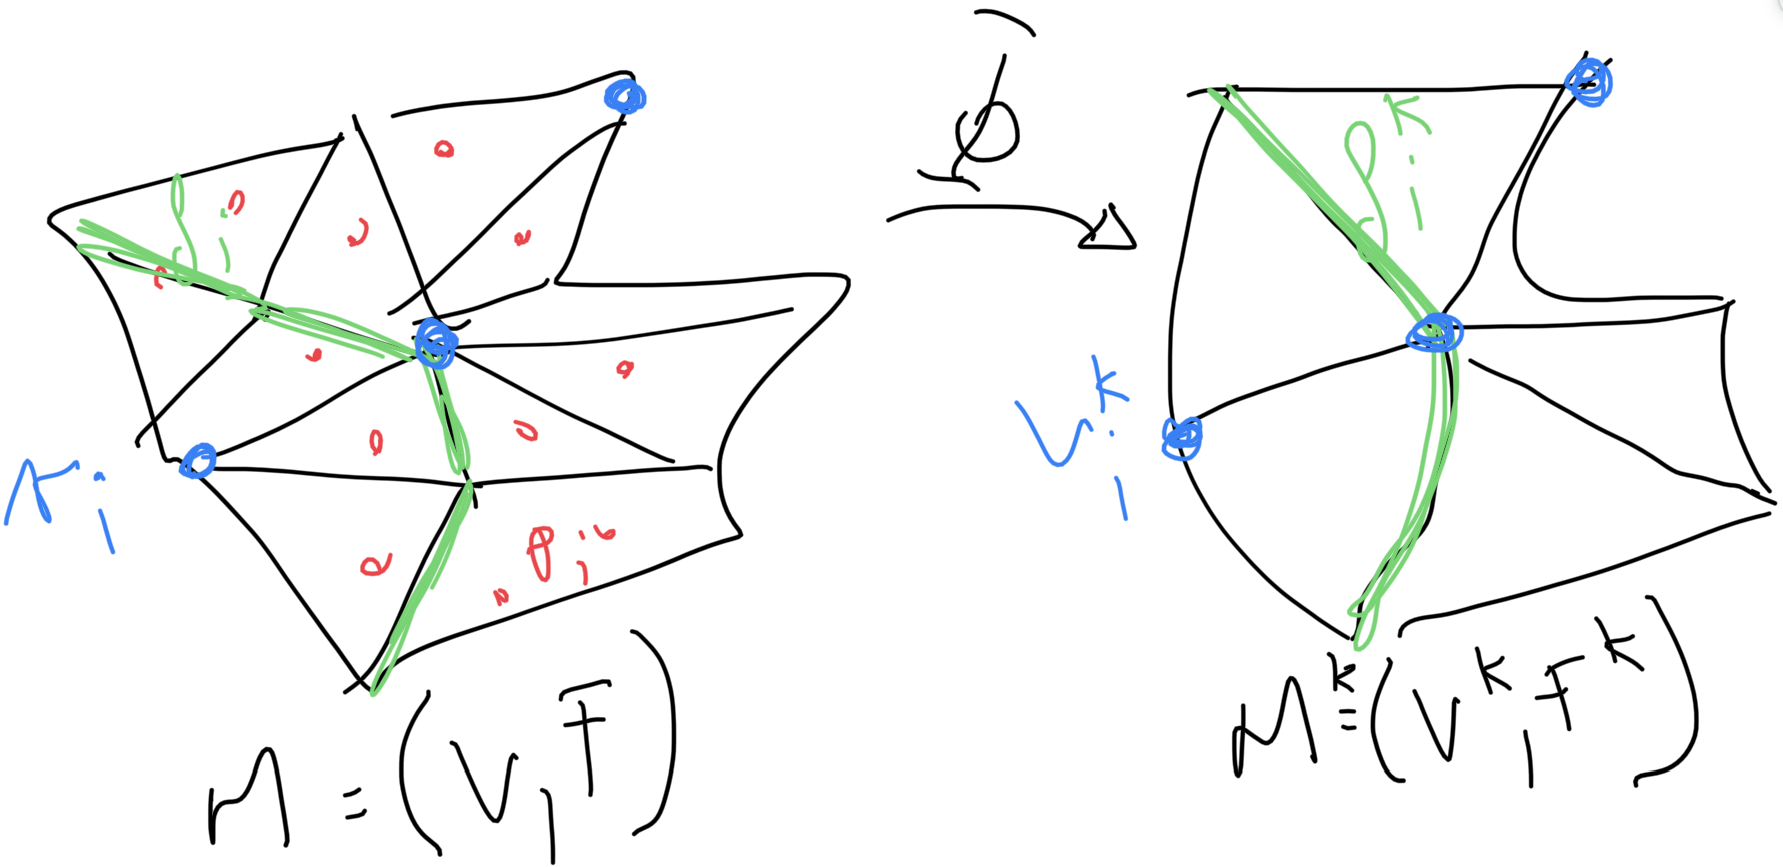
\includegraphics[width=.7\linewidth]{curve_meshing_in_shell_tex/figs/input-output}
    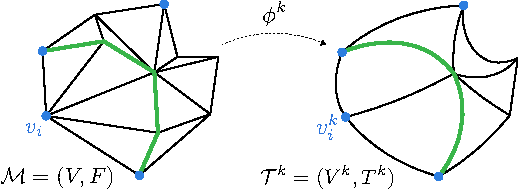
\includegraphics[width=.75\linewidth]{curve_meshing_in_shell_tex/figs/illustrations/input-output-feature.pdf}
    \caption{Input triangle mesh with features and output curved mesh with feature preserved equipped with bijective map $\phi^k$.}
    \label{bichon:fig:input-output-feature}
\end{figure}

% We are now ready to extend the previous construction to features. 
\paragraph{Input}
We enhance the input to additionally include a set of feature edges $f_i\in\F$ and feature vertices $v_i\in\V$ such that no triangle in $F$ has more than one feature edge (Figure~\ref{bichon:fig:input-output-feature} left). (This property can be satisfied on any generic mesh by performing 1-to-3 refinement on every triangle with more than one feature edge). 

\paragraph{Output}
Since the input has features, the output curved mesh $\T^k$ will also have curved {feature} edges $f_i^k\in\T^k$, feature vertices $v_i^k\in\V^k$, and the bijective map $\phi^k$ preserves features by bijectively mapping $\F$ to $\F^k$ and $\V$ to $\V^k$. Our {method} makes no assumption on the topology and ``quality'' of the features. If the features are reasonable, it will produce {a} high-quality mesh, while if the features are close our algorithm will preserve them and result in smaller triangles on the surface. (Figure~\ref{bichon:fig:bad-features}).

\begin{figure}
    \centering
    % \includegraphics{}
    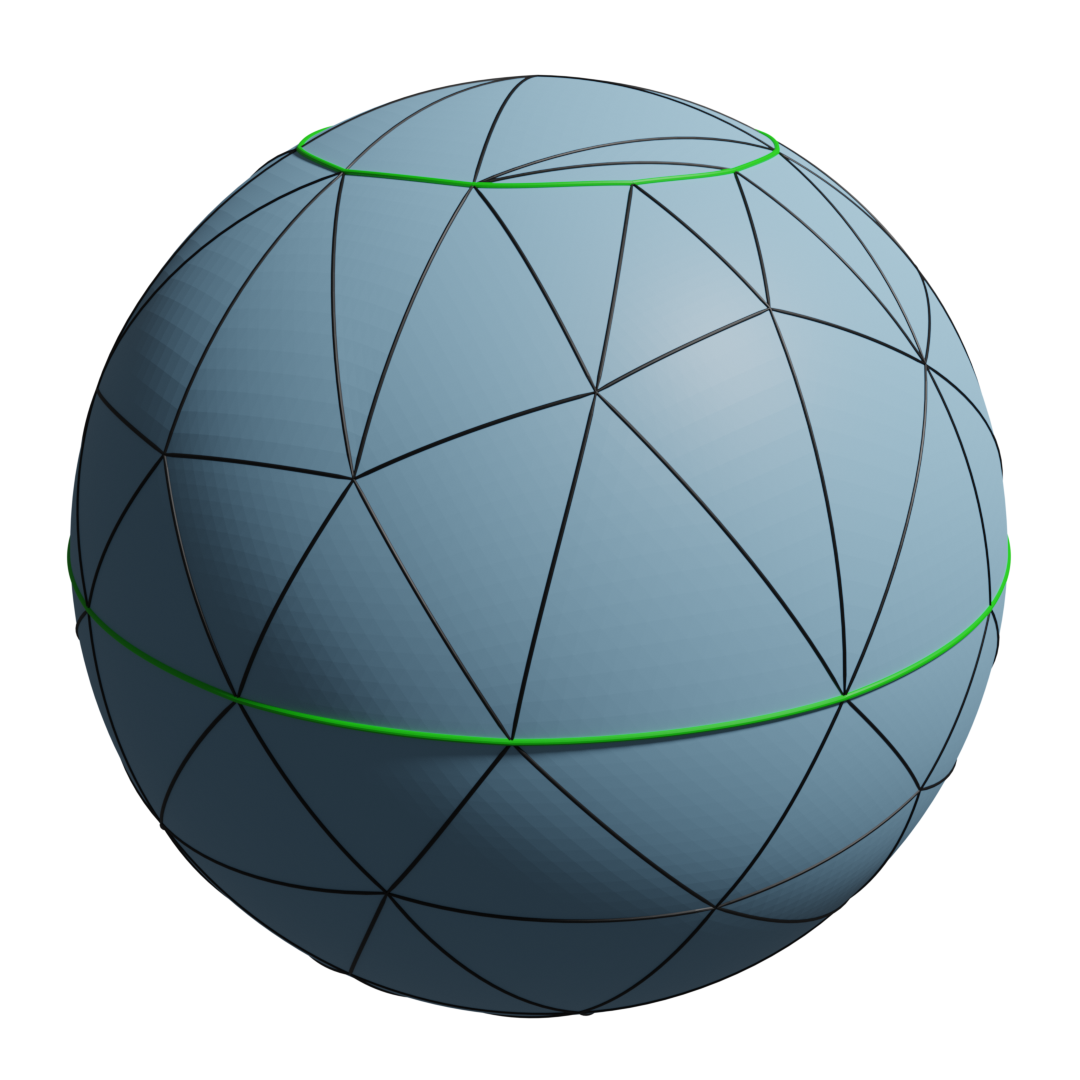
\includegraphics[width=.24\linewidth]{curve_meshing_in_shell_tex/figs/sphere/0001}\hfill
    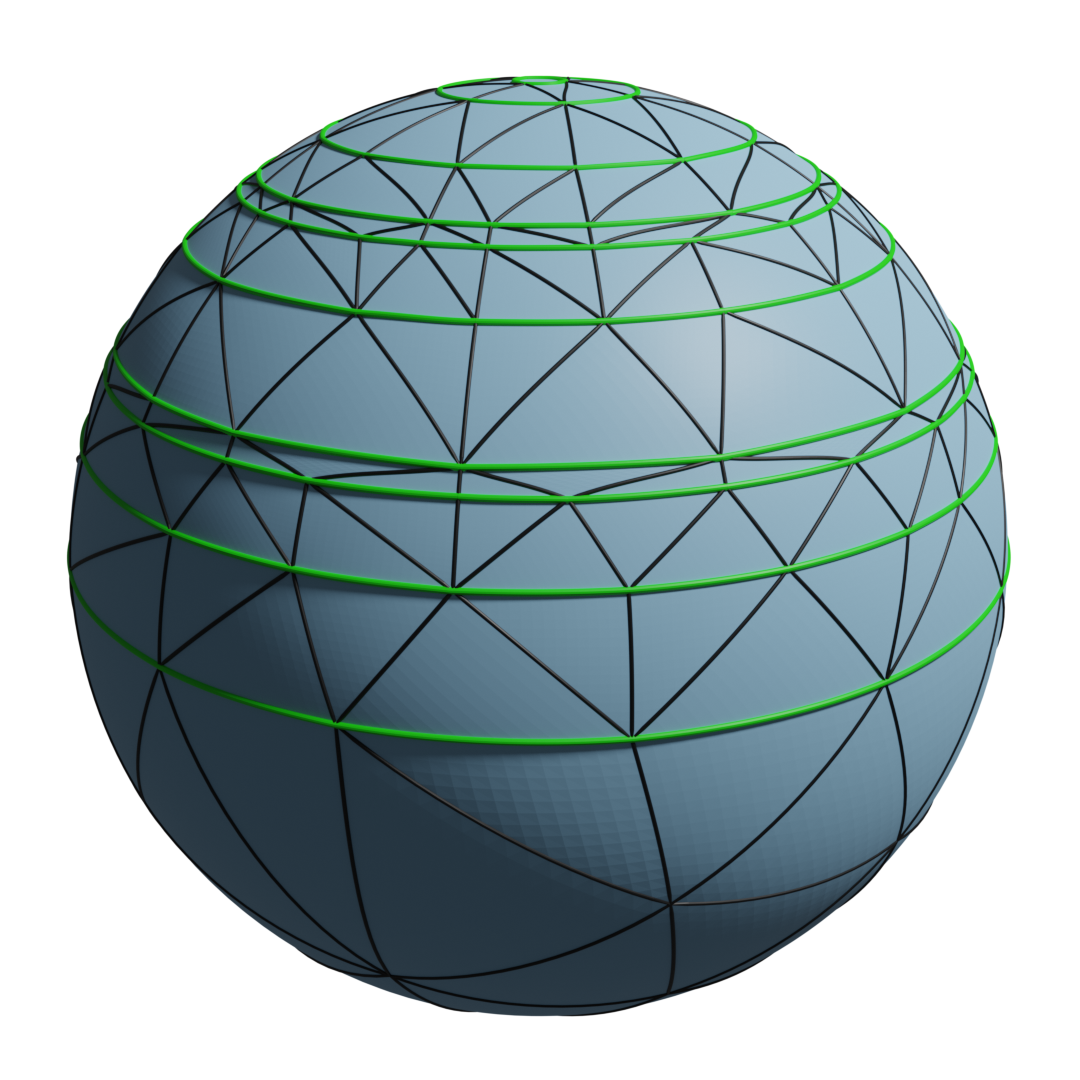
\includegraphics[width=.24\linewidth]{curve_meshing_in_shell_tex/figs/sphere/0002}\hfill
    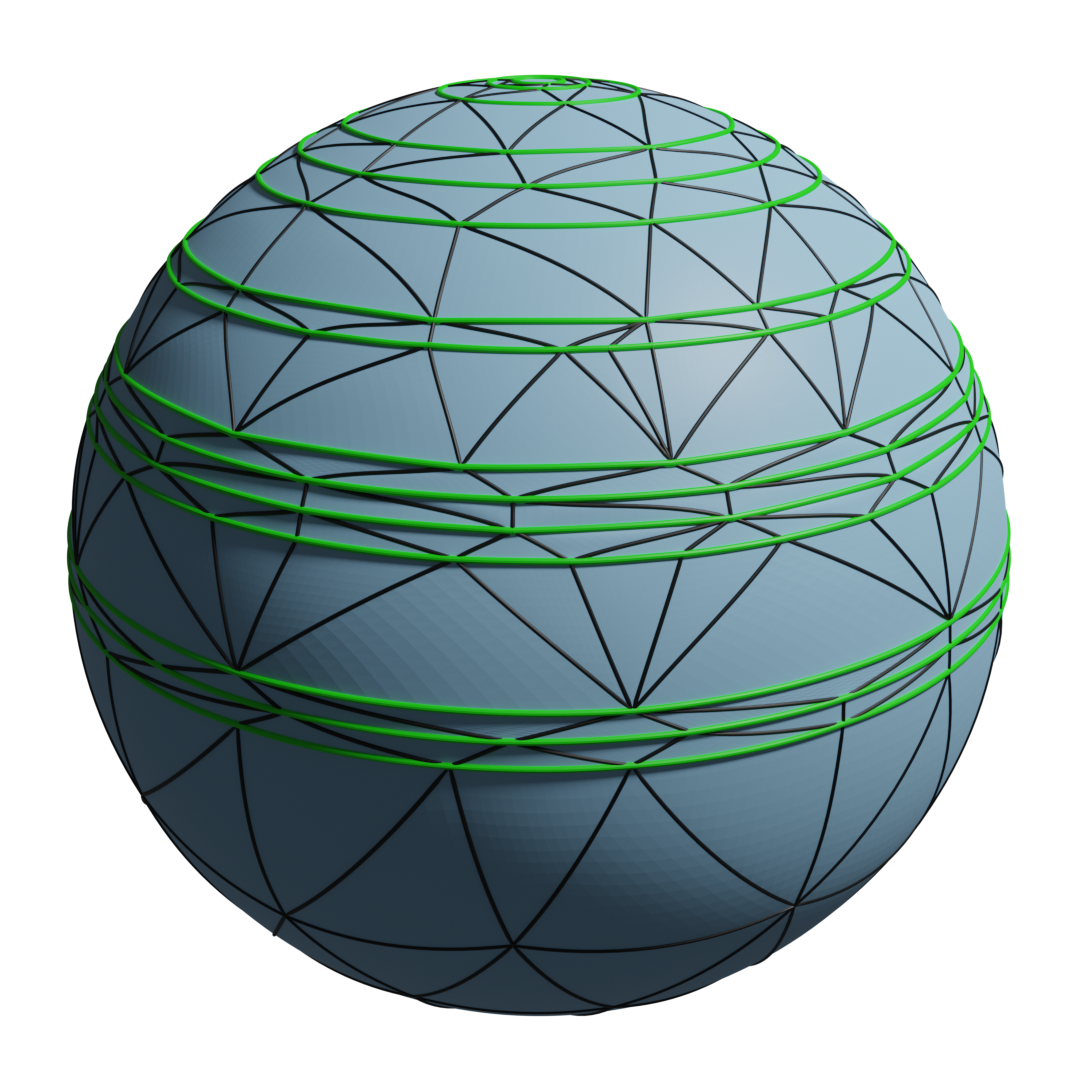
\includegraphics[width=.24\linewidth]{curve_meshing_in_shell_tex/figs/sphere/0003}\hfill
    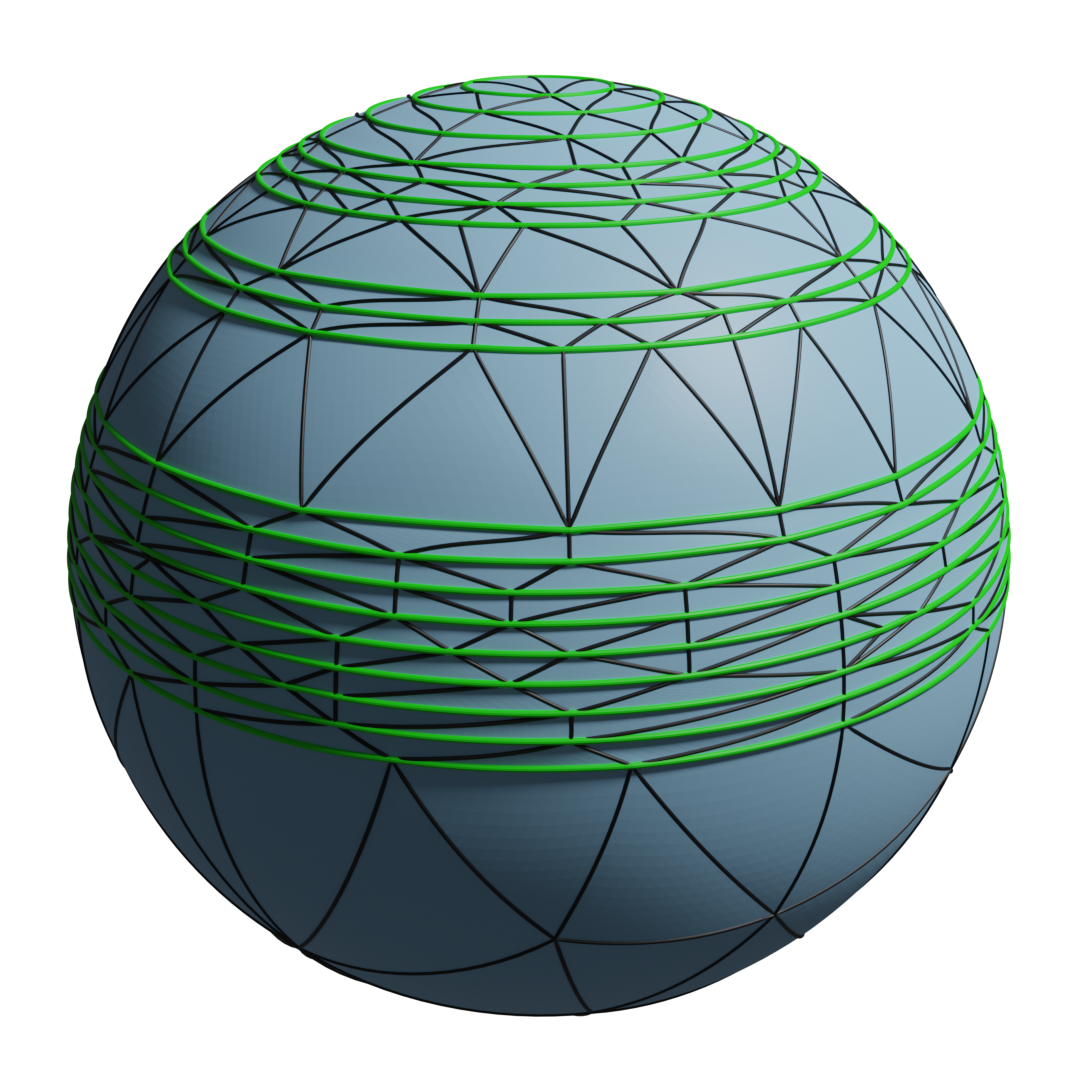
\includegraphics[width=.24\linewidth]{curve_meshing_in_shell_tex/figs/sphere/0004}
    \caption{A sphere with different marked features (green). As we increase the number of features our algorithm will preserve them all but the quality of the surface suffers.}
    \label{bichon:fig:bad-features}
\end{figure}


\begin{figure}
    \centering
    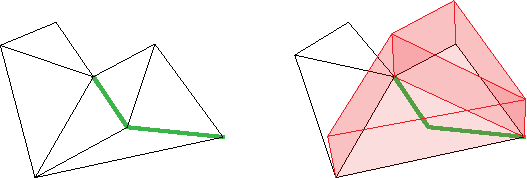
\includegraphics[width=.7\linewidth]{curve_meshing_in_shell_tex/figs/illustrations/not-feat-pres.pdf}
    \caption{Input feature (green) is not preserved after traditional shell simplification.}
    \label{bichon:fig:not-feat-pres}
\end{figure}

The previous construction generates valid curved tetrahedral meshes and the bijective map $\phi^k$ based on the construction of~\cite{jiang2020bijective}. However, the shell construction cannot coarsen features{:} the authors suggest {freezing} them. For instance, when performing an edge collapse on the feature, the new coarse edge (orange) will not map to the feature (green) anymore (Figure~\ref{bichon:fig:not-feat-pres}). 
To ensure feature preservation we extend Definition~\ref{def:curved-mesh}.
\begin{definition}\label{def:curved-features}
We call a curved mesh $\T^K$ and its mapping $\phi^k$ from $\M$ \emph{valid and feature preserving} if they are valid (Definition~\ref{def:curved-mesh}) and $\phi^k$ bijectively maps $\F$ to $\F^k$ and $\V$ to $\V^k$
\end{definition}
As for the non-feature preserving case, we always aim to maintain a valid feature preserving $\T^k$.


\begin{figure}
    \centering
    % 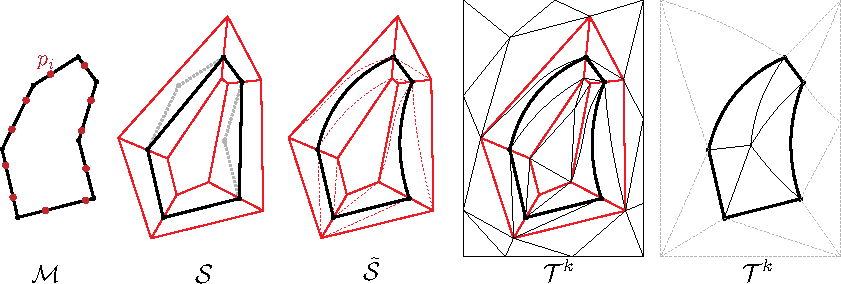
\includegraphics[width=\linewidth]{curve_meshing_in_shell_tex/figs/pipeline}
    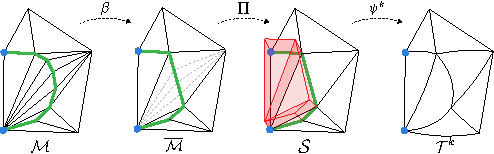
\includegraphics[width=\linewidth]{curve_meshing_in_shell_tex/figs/illustrations/stage-1.pdf}
    \caption{Overview of the construction of the first stage of our pipeline.}
    \label{bichon:fig:stage-1}
\end{figure}

\begin{figure}
    \centering
    % 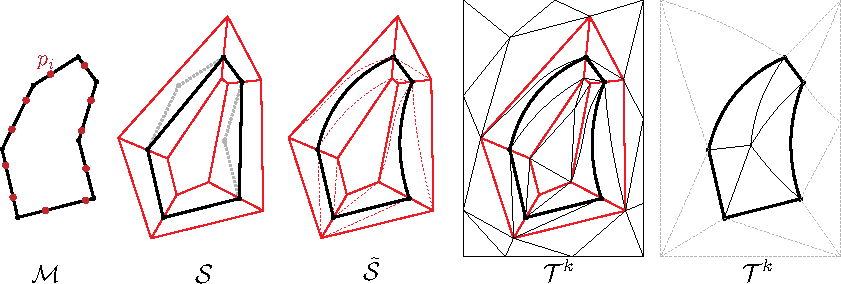
\includegraphics[width=\linewidth]{curve_meshing_in_shell_tex/figs/pipeline}
    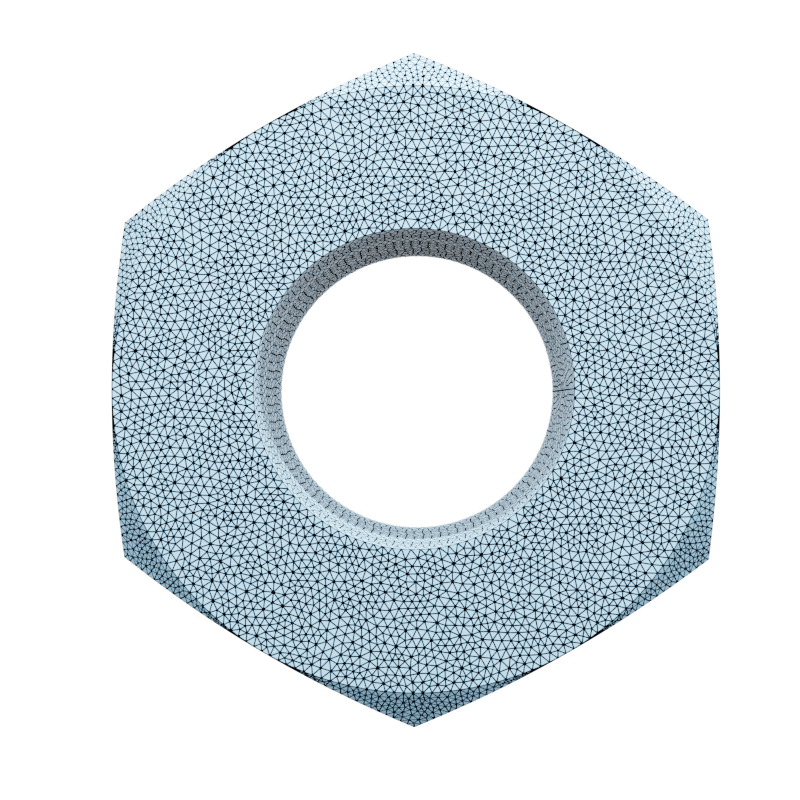
\includegraphics[width=0.33\linewidth]{curve_meshing_in_shell_tex/figs/snap_abc6/0001.png}\hfill
     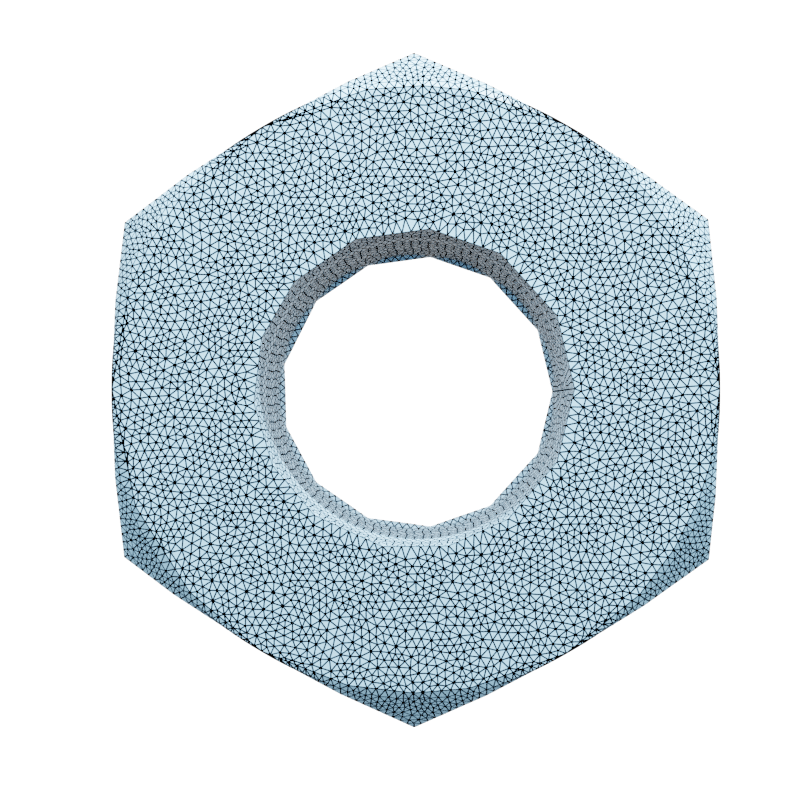
\includegraphics[width=0.33\linewidth]{curve_meshing_in_shell_tex/figs/snap_abc6/0002.png}\hfill
     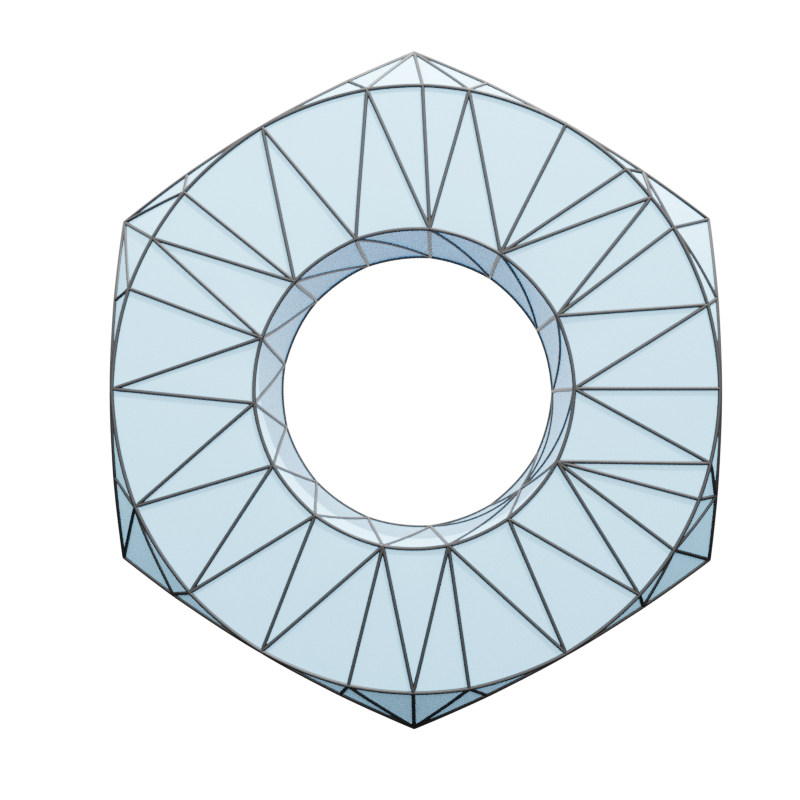
\includegraphics[width=0.33\linewidth]{curve_meshing_in_shell_tex/figs/snap_abc6/0003.png}\par
     \parbox{.33\linewidth}{\centering Input mesh}\hfill
     \parbox{.33\linewidth}{\centering Snapped mesh}\hfill
     \parbox{.33\linewidth}{\centering Curved mesh}
    \caption{The input mesh has feature edges snapped, to create a valid shell, as well as the curved mesh.}
    \label{bichon:fig:ex-snapping}
\end{figure}

To account for features, we propose to change the prismatic map $\Pi$, that is, we only need to change the first stage. This is done by snapping the input features  (Section~\ref{cumin:sec:snapping}). That is, we modify $\M$ to ``straighten'' the feature to ensure that the coarse prismatic projection preserves them and construct a mapping $\beta$ between the {straight} mesh $\overline\M$ and $\M$ (Figure~\ref{bichon:fig:ex-snapping}). 

The outcome {is} a \emph{valid} shell $\PS$ with respect to the {straight} surface $\overline\M$ (i.e., $\overline\M$ is a section $\PS$) that preserve features, the prismatic projection $\Pi$, and the bijective map $\beta$ that can be directly used in the curved pipeline (Section~\ref{cumin:sec:curved-pipeline}). That is, the mapping  $\phi^k$ will be defined as $\phi^k = \beta \circ \Pi \circ \psi^k$.

As for the non-preserving feature pipeline we ensure that our conditions are always met, starting {from} a trivial input and rejecting operations violating them. Our goal is to modify the input mesh $\M$ and create $\overline\M$ by moving its vertices. In such a way, the mapping $\beta$ is simply barycentric. To guarantee bijectivity of $\phi^k$ we need to ensure that all {mappings} composing it are bijective, in particular $\beta$. To ensure that $\beta$ is bijective it is enough that $\overline\M$ is self-intersection free (guaranteed by the shell construction) and that all its triangles have positive area. By straightening the features of $\M$ we ensure that the edges of the prism will map to the feature. Thus, $\phi^k$ will be feature preserving.


\begin{figure}
    \centering
    % \includegraphics[width=0.5\linewidth]{curve_meshing_in_shell_tex/figs/feat-gr}
    \includegraphics[width=0.65\linewidth]{curve_meshing_in_shell_tex/figs/illustrations/feat-gr.pdf}
    \caption{The input edges feature (green) are grouped together in poly-lines and categorized in graph (left) and loops (right). For every graph we add the nodes (blue) to the set of feature vertices.}
    \label{bichon:fig:feat-gr}
\end{figure}

\paragraph{Feature Grouping.}
The first step of our pipeline consists of grouping successive edges $f_i\in\F$ into poly-lines and identifying two categories: loops and graphs (Figure~\ref{bichon:fig:feat-gr}). For every graph, we identify its nodes and add them as feature vertices. In other words, we add to $\V$ all the end-points and junction of poly-lines.


%%%%%%%%%%%%%%%%%%%%%%%%%%%%%%%%%%%%%%%%%%%%%%

\subsection{Feature straightening.}\label{cumin:sec:snapping}
To allow feature coarsening, we propose to straighten $\M$ to ensure that all features are collinear. In other words, we build, together with the shell $\PS$, a mesh $\overline\M = (\overline V,F)$ (i.e., a mesh with the same connectivity $F$ of $\M$) and features $\overline \F$ such that every triangle of $\overline \M$ has a positive area, $\overline \M$ is a section of $\PS$, and the features in $\overline\F$ are collinear. 
In such a way, the mapping $\beta$ is trivially defined as piecewise affine ($\overline\M$ and $\M$ share the same connectivity) and is locally injective as long as all the triangles on $\overline\M$ have positive {areas}. Note that the bijectivity of $\beta$ follows from the fact that the shell prevents self-intersections of $\overline\M$.


\begin{figure}
    \centering
    % 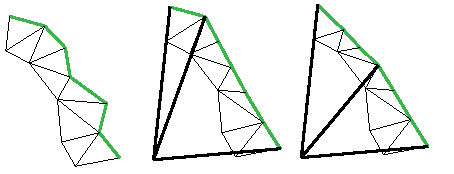
\includegraphics{curve_meshing_in_shell_tex/figs/slide_on_feature.pdf}
    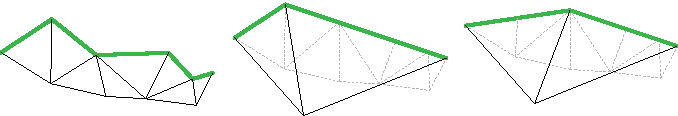
\includegraphics[width=\linewidth]{curve_meshing_in_shell_tex/figs/illustrations/loc-op.pdf}
    \caption{Illustration of smoothing on a feature.}
    \label{bichon:fig:loc-op}
\end{figure}

To construct a mesh $\overline\M$ with straight features, 
we start with $\overline\M = \M$ (in the beginning all prisms of $\PS$ cover at most one feature edge).
Let $\overline f^1 = \{\overline f_i^1\}, i=1,\dots,n$ and $\overline f^2 = \{\overline f_i^2\}, i=1,\dots,k$ two chains of {feature} edge belonging to the same feature $\overline f \in \overline\F$.
For every local operation acting on a feature $\overline f_1$ and $\overline f_2$  we first construct the new feature $\overline f^n = \{\overline f_i^n\}, i=1,\dots,k$ such that the segments $(\overline f_i^n, \overline f_{i+1}^n)$ are collinear and their length is proportional to $( f_i, f_{i+1})$ (the feature vertices in the input mesh $\M$), that this we use arc-length cross parameterization from $f$ to $\overline f^n$ (Figure~\ref{bichon:fig:loc-op} show an example of smoothing a feature). Moving vertices of $\overline f^n$ will also move the vertices of $\overline\M$ thus, straighten the mesh as the local operations {proceed}. After the construction of $\overline f^n$ we check if the newly constructed $\overline\M$ is still a section of $\PS$ and if the triangles modified by the straightening have {areas} larger than  $\epsilon$. In practice, we choose $\epsilon=10^{-10}$: a smaller value would lead to numerical instabilities and a larger one to less straightening.

Note that not all features can be {straight}; for instance, if a triangle has three feature vertices (the snapped feature will result {in} a degenerate triangle, thus, $\beta$ will not be bijective) or if the snapping flips the normal ($\overline\M$ will no longer be a section of $\PS$). Both are extremely rare cases in our dataset.
%%%%%%%%%%%%%%%%%%%%%%%%%%%%%%%%%%%%%%%%%%%%%%

